
\chapter{Lo \textit{stage}}
\label{cap:lo-stage}



\section{Il ruolo degli stage nell'azienda}
Zero12 crede fortemente nella collaborazione tramite \textit{stage} con gli studenti dell'Università di Padova. Grazie all'evento \gls{stageItg}, un' evento promosso da Confindustria Veneto Est e l'Universita degli studi di Padova, l'azienda permette agli studenti di svolgere progetti di \textit{stage} presso la loro sede.
Gli stage per l'azienda, rappresentano una doppia opportunità. Da una parte, hanno modo di inserire nuove figure professionali nel proprio organico, dall’altra gli studenti hanno la possibilità di inserirsi nel mondo del lavoro e poter applicare le proprie conoscenze acquisite durante il percorso di studi.
Durante le otto settimane di \textit{stage} ho avuto l’occasione di conoscere quasi tutti i membri dell’azienda, comprendere il loro metodo di lavoro e mettere in pratica le mie conoscenze. Il mio percorso è stato guidato dal \textit{tutor} aziendale, che mi è stato assegnato, coordinando le varie attività da svolgere e fornendo supporto in caso di dubbi o problemi. 
L'accoglienza e l'ambiente di lavoro sono molto positivi, dimostrando una grande attenzione nei confronti degli stagisti. 
Questa attenzione, è testimoniata anche dalla presenza di molti dipendenti che attualmente lavorano in azienda dopo aver svolto uno \textit{stage} in Zero12.
I progetti assegnati durante gli \textit{stage} vengono concepiti in base a delle reali esigenze interne all’azienda. Essi sono mirati a migliorare la comunicazione tra i collaboratori, automatizzare delle attività manuali e a migliorare la qualità del lavoro svolto.

\section{Introduzione al progetto}
Durante il mio \textit{stage} ho avuto modo di lavorare non solo al progetto inizialmente proposto, ma anche allo sviluppo di progetto aggiuntivo, strettamene correlato al primo.
Di seguito descrivo il progetto inizialmente proposto dall'azienda all'evento \gls{stageItg} e il progetto aggiuntivo concepito e sviluppato durante lo \textit{stage}.
\subsection{Sistema di proposte di risoluzioni a \textit{ticket} Jira} \label{sec:spiegazioneJira}
L'idea del progetto nasce come strumento che l'azienda può utilizzare per velocizzare il supporto tecnico, che però può essere estesa ai clienti dell'azienda stessa. Nel contesto del progetto, viene immaginata un'azienda che vende componenti \textit{hardware}. 
Nel caso di problematiche con la componente comprata, il cliente chiama il servizio clienti dell'azienda, e l'operatore inserisce un \textit{ticket} all'interno dell'\gls{its} aziendale, Jira nel contesto del progetto. Immaginando questa iterazione tra cliente e addetto al servizio clienti per molte volte nel corso degli anni, i \textit{ticket} inseriti all'interno del sistema saranno numerosi e molto simili tra loro. 
Questo proietta al fatto che a nuovi \textit{ticket} inseriti, molto probabilmente ci saranno dei \textit{ticket} simili già risolti in passato. 
Ed è qui che da Zero12 nasce l'idea di creare un sistema di proposte di risoluzioni automatiche di \textit{ticket} inseriti all'interno di un \gls{its}, che permetta di velocizzare il processo di risoluzione del problema. Le proposte di risoluzione vengono generate grazie all'utilizzo della IA Generativa, in base al contesto dei \textit{ticket} completati in precedenza.

\begin{figure}[H]
    \centering
    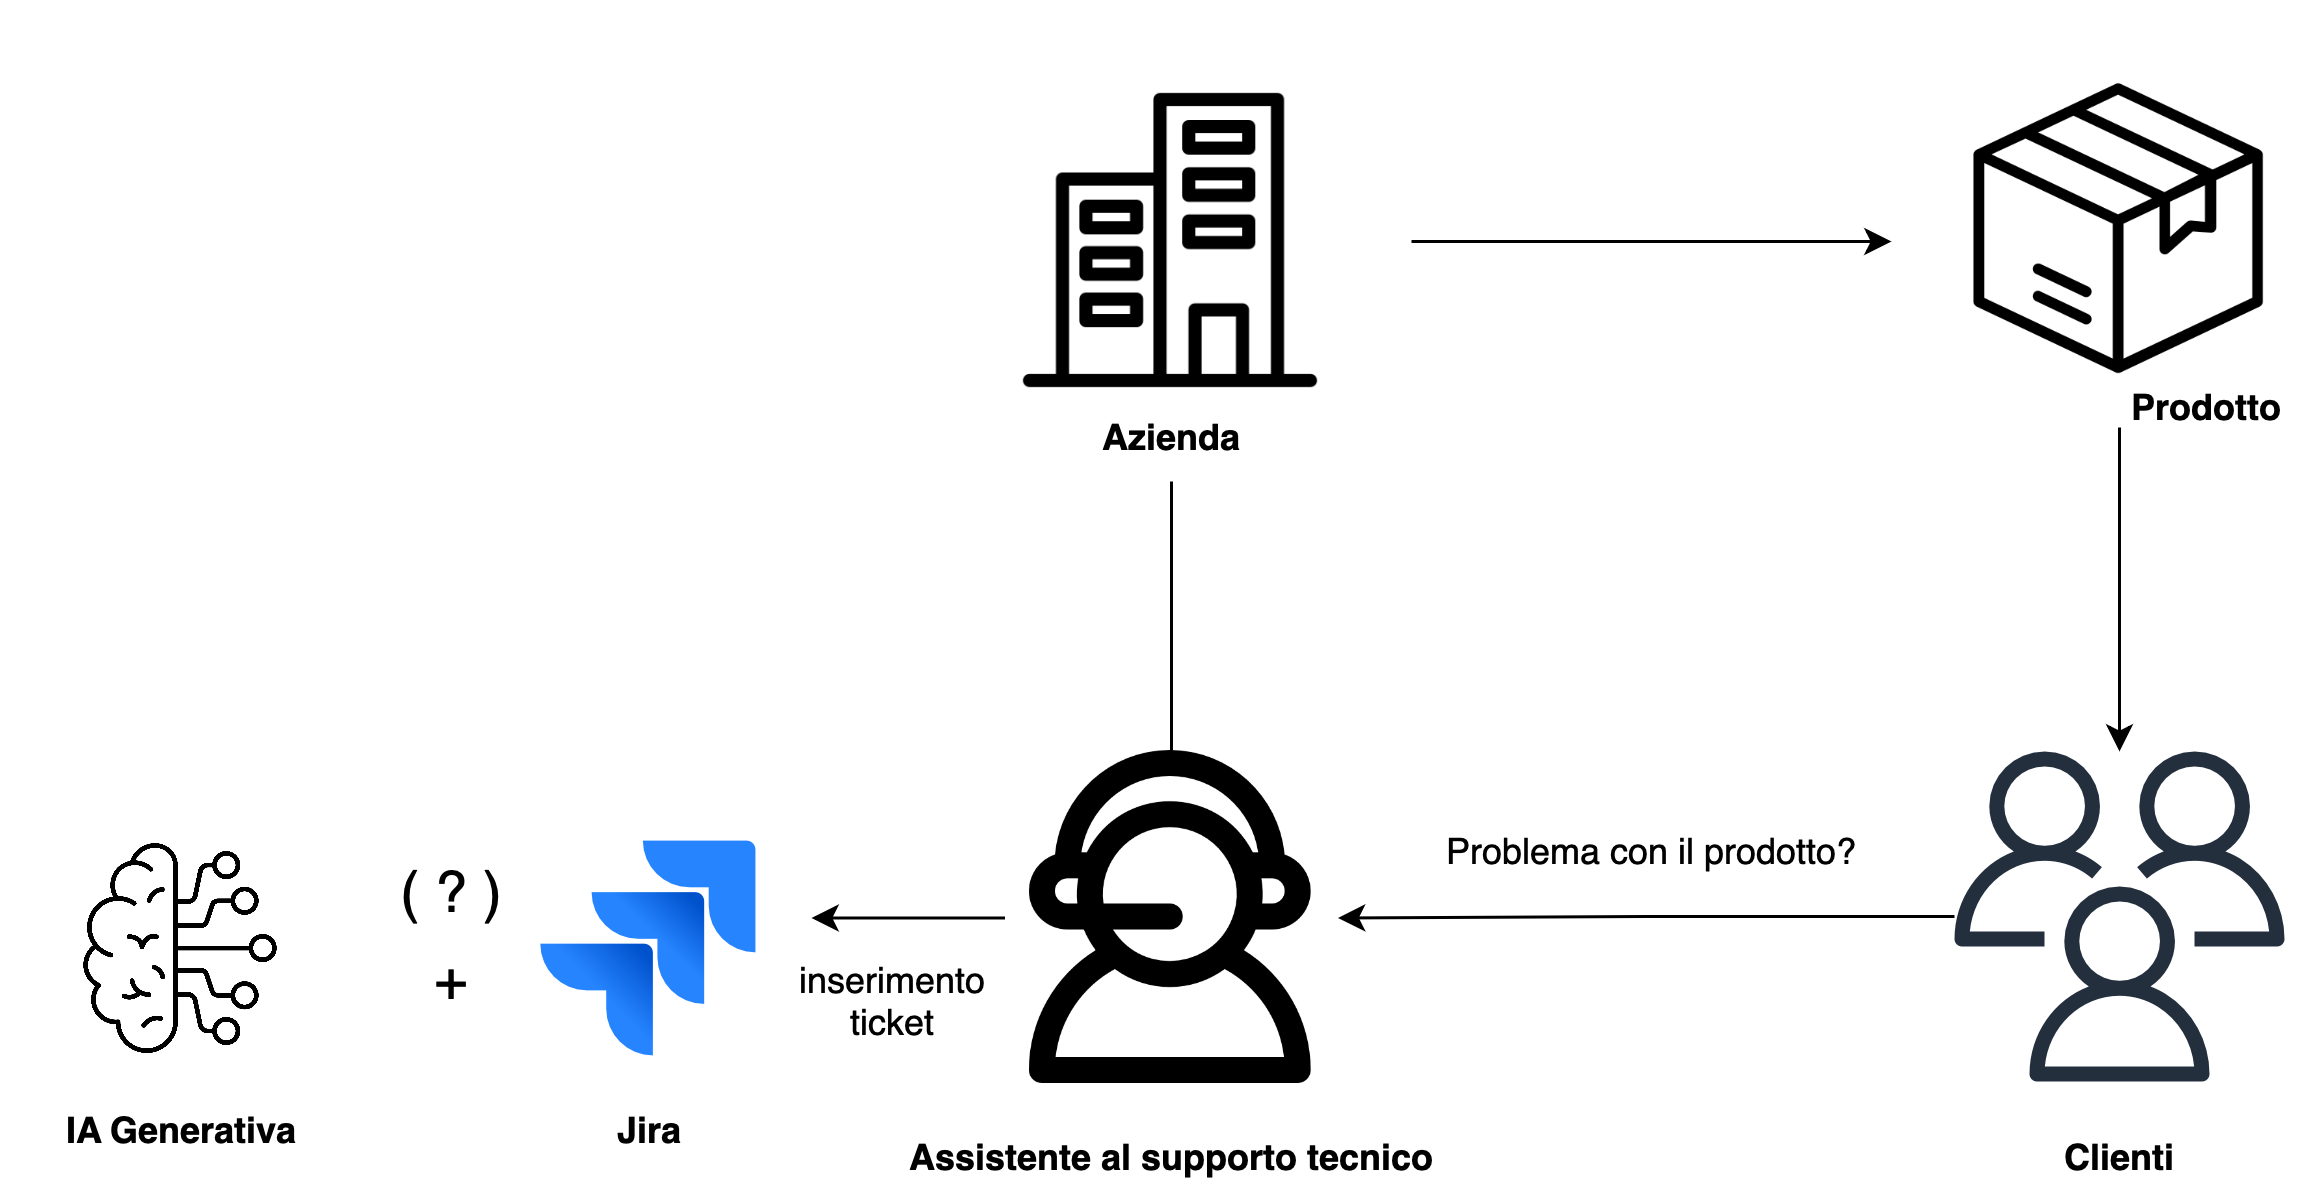
\includegraphics[width=0.85\textwidth]{ideaJira.png}
    \caption{Schema che rappresenta l'idea del progetto principale}
    \small \textbf{Fonte:} \href{https://www.flaticon.com/free-icon/company_4812244}{Icona azienda: https://www.flaticon.com} \href{https://www.flaticon.com/free-icon/box_4601560}{Icona prodotto: https://www.flaticon.com} \href{https://www.flaticon.com/free-icon/assistant_1442194}{Icona assistente: https://www.flaticon.com} \href{https://www.creativefabrica.com/it/product/ai-brain-outline-icon/} {Icona IA Generativa: https://www.creativefabrica.com}

    \label{fig:ideaJira}
\end{figure}
\subsection{\textit{Chatbot} per proposte di risoluzioni}
Durante lo sviluppo del progetto descritto nel paragrafo precedente, è nata l'idea di creare un ulteriore strumento che permetta di svolgere la stessa funzionalità del sistema di proposte di risoluzioni, ma in modo differente. Lo strumento aggiuntivo è un \textit{chatbot} che permette di generare proposte di risoluzione, in base al testo di un \textit{ticket} inserito all'interno della chat. 
Sempre grazie all'utilizzo della IA Generativa, il \textit{chatbot} genera proposte di risoluzione in base al contesto dei \textit{ticket} completati in precedenza. A differenza del sistema Jira, il \textit{chatbot} propone le risoluzioni in modo più descrittivo e dettagliato, e permette di interagire con l'assistente virtuale, per ottenere informazioni più dettagliate sulle proposte di risoluzione.
\begin{figure}[H]
    \centering
    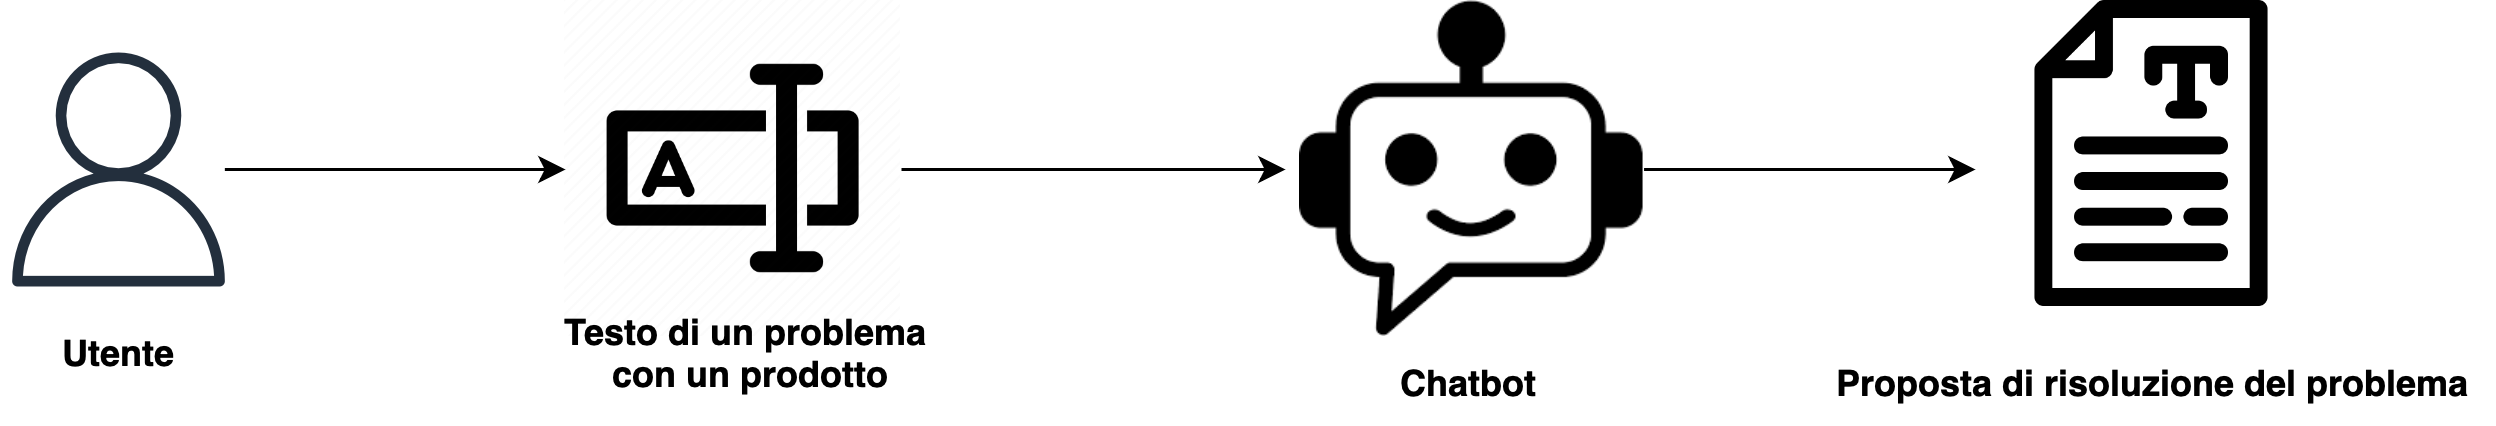
\includegraphics[width=0.85\textwidth]{ideaChatbot.png}
    \caption{Schema che rappresenta l'idea del progetto aggiuntivo}
    \label{fig:ideaChatbot}
    \small \textbf{Fonte:} \href{https://uxwing.com/chatbot-icon/}{Icona chatbot: https://uxwing.com} \href{https://www.iconfinder.com/icons/351012/field_input_search_icon}{Icona \textit{input} : https://www.iconfinder.com} \href{https://www.flaticon.com/free-icon/text-file_5116156} {Icona testo: https://www.flaticon.com}

\end{figure}
\section{Importanza del progetto}
Come descritto nel paragrafo precedente, il progetto ideato da Zero12 di generare proposte di risoluzioni automatiche per i nuovi \textit{ticket} inseriti all'interno di un \gls{its} rappresenterebbe un grande vantaggio per l'azienda. Innanzitutto, 
grazie allo sviluppo di questo progetto, l'azienda ha dei dati sufficienti per poter implementare un sistema di proposte di risoluzioni automatiche, utilizzando i servizi di cui l'azienda è \textit{partner}. In secondo luogo, permette di avere un'idea nel 
caso un cliente, voglia implementare un sistema simile a quello sviluppato. Questo permetterebbe di avere già un prototipo funzionante, che mostra tutte le potenzialità del sistema, e che può essere facilmente adattato al contesto aziendale del cliente.
Questo perchè l'utilizzo di IA Generativa sta diventando sempre più utilizzato in ambito aziendale, data la sua capacità di generare risposte in base al contesto in cui viene inserita.
Riguardo al progetto aggiuntivo, la creazione di un \textit{chatbot} per le proposte di risoluzione ha la stessa importanza del progetto principale. 

\section{Obiettivi dello \textit{stage}}
Durante i primi giorni di \textit{stage} ho definito assieme al mio \textit{tutor} aziendale gli obiettivi del progetto.
Di seguito nella tabella elenco gli obiettivi da raggiungere:
\renewcommand{\arraystretch}{2}
\begin{longtable}{|p{10cm}|p{2cm}|}
    \hline
    \rowcolor{tableheader}\textbf{Obiettivo} & \textbf{Importanza} \\
    \hline
    \endfirsthead

    \rowcolor{tableheader}\textbf{Obiettivo} & \textbf{Importanza} \\
    \hline
    \endhead

    \hline
    \endfoot

    \hline
    \endlastfoot
    \rowcolor{tableoddrow} Studio delle tecnologie e studio di fattibilità & Obbligatorio \\
    \hline
    \rowcolor{tableevenrow} Creazione dati di \textit{mock} da inserire nell' \gls{its} Jira & Obbligatorio \\
    \hline
    \rowcolor{tableoddrow} Reperimento dei ticket su Jira e salvataggio su \textit{database} mongoDB & Obbligatorio \\
    \hline
    \rowcolor{tableoddrow} Aggiornamento costante del \textit{database} a nuovi \textit{ticket} chiusi su Jira & Obbligatorio \\
    \hline
    \rowcolor{tableoddrow} Esecuzione di \gls{rag}, una tecnica avanzata di elaborazione di linguaggio naturale, sui \textit{ticket} salvati & Obbligatorio \\
    \hline
    \rowcolor{tableoddrow} Creazione del sistema di proposte di risoluzione su Jira & Obbligatorio \\
    \hline
    \rowcolor{tableoddrow} \textit{Benchmark} su vari modelli per la generazione della risposta & Desiderabile \\
    \hline
    \caption{Obiettivi da raggiungere per il sistema di proposte di risoluzione su Jira}
    \label{tab:obiettiviJira}
\end{longtable}
\noindent
Durante lo sviluppo del progetto, visto il buon andamento che ho avuto, insieme al mio \textit{tutor} aziendale è nata l'idea di sviluppare un progetto aggiuntivo, ovvero il \textit{chatbot} per le proposte di risoluzione.
Di seguito nella tabella elenco gli obiettivi \textit{extra} da raggiungere:
\begin{longtable}{|p{10cm}|p{2cm}|}
    \hline
    \rowcolor{tableheader}\textbf{Obiettivo} & \textbf{Importanza} \\
    \hline
    \endfirsthead

    \rowcolor{tableheader}\textbf{Obiettivo} & \textbf{Importanza} \\
    \hline
    \endhead

    \hline
    \endfoot

    \hline
    \endlastfoot
    \rowcolor{tableoddrow} Studio delle tecnologie e studio di fattibilità & Desiderabile \\
    \hline
    \rowcolor{tableevenrow} Implementazione interfaccia \textit{web} per l'interrogazione del \textit{chatbot} & Desiderabile \\
    \hline
    \rowcolor{tableevenrow} Impostazione di un formato di domanda dell'utente da seguire & Desiderabile \\
    \hline
    \caption{Obiettivi da raggiungere del progetto \textit{chatbot}}
    \label{tab:obiettiviChatbot}
\end{longtable}
\section{Vincoli dello \textit{stage}}
\subsection{Vincoli tecnologici}
I vincoli tecnologici imposti dall'azienda consistevano nell'utilizzo delle tecnologie utilizzata nello \textit{stack} aziendale, come sono riportate nella sezione \ref{sec:tecnologie}. In aggiunta a queste, 
mi è stato chiesto di usufruire delle \gls{api} che fornisce Jira, per il caricamento dei \textit{ticket} di \textit{mock} all'interno di un progetto Jira, e per il recupero dei \textit{ticket} completati da inserire all'interno del \textit{database}
Mi è stato inoltre chiesto di utilizzare i \textit{webhook} di Jira, per poter impostare un \textit{trigger} che possa inviare eventi al sistema che ho sviluppato, in cui, in caso di chiusura di un \textit{ticket} su Jira, il sistema aggiorna automaticamente il \textit{database}.
\subsection{Vincoli di rendicontazione}
Durante il mio periodo di \textit{stage}, l'azienda mi ha richiesto la stesura di una tabella, risultato del \textit{benchmark} dei vari modelli testati. Questa tabella doveva contenere i risultati ottenuti dai vari modelli, secondo le metriche di valutazione da me impostate e motivate.
La stesura di un documento in cui spiego le scelte adottate durante lo sviluppo del progetto, indicando le componenti sviluppate, le librerie utilizzate e le motivazioni dietro le scelte fatte.
La stesura di un manuale utente, in cui spiego come impostare correttamente il sistema su Jira, e come utilizzarlo. Quest'ultimo documento comprende anche il corretto utilizzo del \textit{chatbot}, indicando il suo corretto utilizzo.
Durante l'ultima settimana infine, mi è stato richiesto di preparare una presentazione dei progetti sviluppati, che avrei dovuto esporre a tutti i membri presenti dell'azienda. Questa presentazione doveva contenere l'idea del progetto, la sua importanza, i risultati ottenuti e le possibile evoluzioni future.
\subsection{Vincoli temporali}
Il progetto di \textit{stage} è stato ideato per essere sviluppato in otto settimane, limite massimo di tempo per lo svolgimento del tirocinio curricolare. Nello specifico, è stato programmato in giornate lavorative da 8 ore ciascuna, per un totale di non più di 320 ore, per un totale di 40 ore settimanali.

\section{Scelta dello \textit{stage}} \label{sec:sceltaStage}
Durante l'evento \gls{stageItg} ho avuto modo di connoscere numerose azienda, e di ascoltare i loro progetti di \textit{stage}. 
La scelta del progetto di Zero12 è stata basata su una serie di fattori che descrivo qui di seguito:
\begin{itemize}
    \item \textbf{Tema del progetto}: Il progetto sul supporto tecnico facilitato con l'aiuto della IA Generativa, come descritto nel paragrafo \ref{sec:spiegazioneJira}, mi ha subito colpito, in quanto mi ha permesso di approfondire l'utilizzo di questa tecnologia, ormai sempre più utilizzata in vari ambiti. Un'altro motivo per cui ho scelto questo progetto, è stata l'utilità che un sistema del genere può avere in ambito aziendale, e la possibilità di poter estendere anche a clienti reali.
    \item \textbf{Prima impressione}: Come ho raccontato all'inizio del paragrafo, ho avuto modo di parlare con diverse aziende. Il colloquio che ho avuto con Zero12 è stato quello che mi è rimasto più impresso, in quanto si sono dimostrati molto disponibili nel rispondere alle mie domande, molto chiari nelle loro descrizioni e molto accoglienti. A seguito del colloquio, e a seguito dell'ottima impressioni che ho ricevuto da loro, mi sono interessato maggiormente al progetto proposto.
    \item \textbf{Tecnologie utilizzate}: I giorni prima dell'evento, ho avuto modo di leggere le tecnologie richieste per lo sviluppo del progetto. Erano presenti tecnologie che già mi erano note, quali ad esempio Typescript, Node.js e MongoDB. Il restante delle tecnologie, erano legate ai servizi \textit{cloud} offerte da \gls{aws}, che ho avuto modo di accennare durante il mio percorso di scuola superiore. La scelta è stata motivata anche dalla possibilità di approfondire queste tecnologie e di poterle utilizzare in un ambito aziendale.
\end{itemize}

\section{Obiettivi personali}
Prima dell'inizio dello \textit{stage}, mi sono prefissato degli obiettivi che volevo raggiungere grazie a questa esperienza, qui di seguito elencati:
\begin{itemize}
    \item \textbf{Approfondimento e apprendimento di nuove tecnologie}: Come ho accennato nel paragrafo \ref{sec:sceltaStage}, ero già familiare con alcune tecnologie o servizi \textit{cloud} richiesti per lo sviluppo del progetto. Tuttavia, non ho mai avuto modo di poter approfondire queste tecnologie, e di poterle utilizzare al loro massimo potenziale. Questo è stato possibile grazie ai membri dell'azienda, con la quale ho avuto modo di confrontarmi.
    \item \textbf{Introduzione al mondo del lavoro}: Questa è stata la mia prima esperienza lavorativa in un'azienda collegata al mio percorso di studi. Ho avuto modo di conoscere alcune realtà aziendali, ma l'esperienza in Zero12 è stata la prima ad offrirmi un'opportunità lavorativa in questo specifico settore. Ho voluto cogliere questa occasione per comprendere come si lavori in questo tipo di aziende, le loro metodologie e la loro organizzazione interna. 
\end{itemize}